\documentclass[12pt,reqno]{article}
\usepackage{amsthm, amsmath, amsfonts, amssymb, amscd, mathtools, youngtab, euscript, mathrsfs, verbatim, enumerate, multicol, multirow, bbding, color, babel, esint, geometry, tikz, tikz-cd, tikz-3dplot, array, enumitem, hyperref, thm-restate, thmtools, datetime, graphicx, tensor, braket, slashed, standalone, pgfplots, ytableau, subfigure, wrapfig, dsfont, setspace, wasysym, pifont, float, rotating, adjustbox, pict2e,array}
\usepackage{amsmath}
\usepackage[utf8]{inputenc}
\usetikzlibrary{arrows, positioning, decorations.pathmorphing, decorations.pathreplacing, decorations.markings, matrix, patterns}
\tikzset{big arrow/.style={
    decoration={markings,mark=at position 1 with {\arrow[scale=1.5,#1]{>}}},
    postaction={decorate},
    shorten >=0.4pt},
  big arrow/.default=black}

\begin{document}

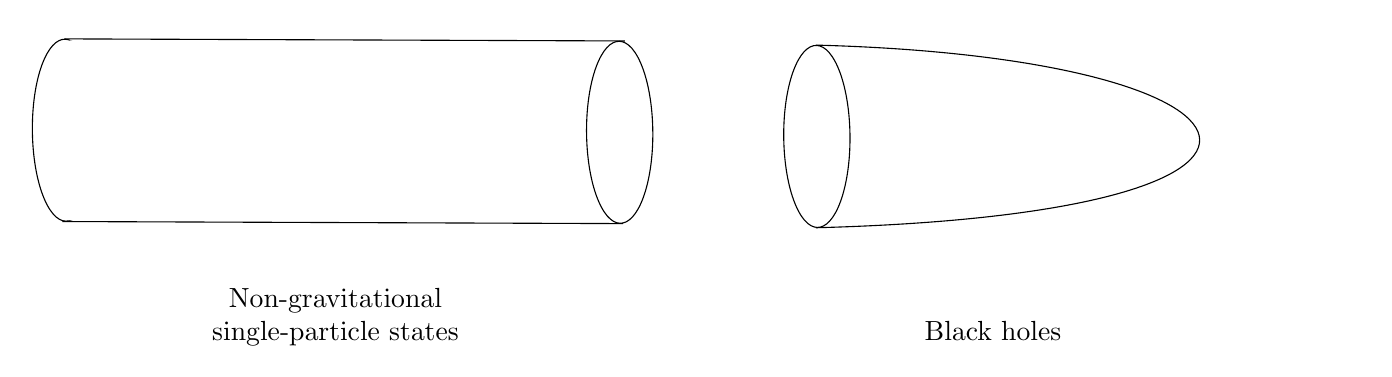
\begin{tikzpicture}[x=0.75pt,y=0.75pt,yscale=-1,xscale=1]

\draw   (40.96,124.53) .. controls (34.1,108.93) and (33.04,81.27) .. (38.58,62.75) .. controls (44.13,44.23) and (54.18,41.87) .. (61.04,57.47) .. controls (67.9,73.07) and (68.96,100.73) .. (63.42,119.25) .. controls (57.87,137.77) and (47.82,140.13) .. (40.96,124.53) -- cycle ;
\draw   (307.96,125.53) .. controls (301.1,109.93) and (300.04,82.27) .. (305.58,63.75) .. controls (311.13,45.23) and (321.18,42.87) .. (328.04,58.47) .. controls (334.9,74.07) and (335.96,101.73) .. (330.42,120.25) .. controls (324.87,138.77) and (314.82,141.13) .. (307.96,125.53) -- cycle ;
\draw    (50.5,47) -- (320.5,48) ;
\draw    (49.5,135) -- (319.5,136) ;
\draw  [color={rgb, 255:red, 255; green, 255; blue, 255 }  ,draw opacity=1 ][fill={rgb, 255:red, 255; green, 255; blue, 255 }  ,fill opacity=1 ] (43.18,122.21) .. controls (36.81,105.71) and (36.51,78.41) .. (42.52,61.23) .. controls (48.53,44.05) and (58.57,43.51) .. (64.94,60.01) .. controls (71.31,76.51) and (71.61,103.82) .. (65.6,120.99) .. controls (59.59,138.17) and (49.56,138.72) .. (43.18,122.21) -- cycle ;
\draw   (402.96,127.53) .. controls (396.1,111.93) and (395.04,84.27) .. (400.58,65.75) .. controls (406.13,47.23) and (416.18,44.87) .. (423.04,60.47) .. controls (429.9,76.07) and (430.96,103.73) .. (425.42,122.25) .. controls (419.87,140.77) and (409.82,143.13) .. (402.96,127.53) -- cycle ;
\draw    (412.5,50) .. controls (641,56) and (676.5,131) .. (412.5,138) ;

% Text Node
\draw (116,166) node [anchor=north west][inner sep=0.75pt]   [align=left] {\begin{minipage}[lt]{95.7pt}\setlength\topsep{0pt}
\begin{center}
Non-gravitational\\single-particle states\\
\end{center}

\end{minipage}};
% Text Node
\draw (460,182) node [anchor=north west][inner sep=0.75pt]   [align=left] {\begin{minipage}[lt]{54.88pt}\setlength\topsep{0pt}
\begin{center}
Black holes
\end{center}

\end{minipage}};


\end{tikzpicture}

\end{document}